\vsssub
\subsubsection{~未解析障碍物} \label{sub:num_obst}
\conthead{\ws}{H. L. Tolman, L. Mentaschi}

\noindent
即使在 \ws\ 1.15 版最初调参时 \citep{tol:OMB02a}，也已清楚未解析岛群是局地波浪模式误差的主要来源。这一点在 \citet[][图~3]{tol:Waves01a} 和 \citet[][图~8]{tol:WaF02} 中有更详细说明。在 \ws\ 中，有两种方法可用于参数化未解析障碍物。第一种方法最初来自 \swan\ \citep{art:BRH99,man:SWAN3}，它在数值格式内部的空间网格单元边界处施加未解析障碍物的影响，并已用于规则网格。第二种方法由 \citep{art:Mentaschi2015b} 提出，基于源项，可应用于不同网格类型。本节介绍第一种方法；第二种方法的说明见第 \ref{sec:UOST} 节。

在基于传播的方法中，通过单元公共边界的数值通量会按照未解析障碍物提供的阻挡程度受到抑制。在该方法中，式~(\ref{eq:uq_xy_tot}) 的 \uq{} 格式数值传播格式修改为

% eq:uq_xy_obstr

\begin{equation}
\cN_{i,j,l,m}^{n+1} = \cN_{i,j,l,m}^n +
\frac{\Delta t}{\Delta \phi} \left [ \alpha_{i,-} \cF_{i,-} - \alpha_{i,+} \cF_{i,+} \right ]
\: , \label{eq:uq_xy_obstr} \end{equation}

\begin{figure} \begin{center}
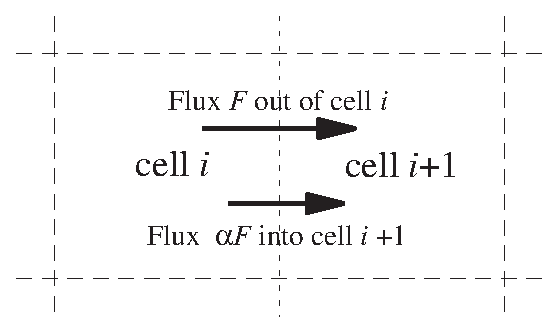
\epsfig{file=./num/obstr.eps,angle=0,width=2.2in}
\caption{未解析障碍物的处理。公共单元边界（点线）的透明度为 $\alpha$。虚线表示其他单元边界。数值通量从左向右。}
         \label{fig:obstr} \botline
\end{center}
\end{figure}

\noindent
其中 $\alpha_{i,-}$ 和 $\alpha_{i,+}$ 是相应单元边界的“透射率”，范围从 0（封闭边界）到 1（无遮挡）。对于出流边界，透明度按定义为 1，否则能量会在单元中人为累积。对于入流边界，小于 1 的透明度会导致受阻能量在单元边界处被移除。该方法如图~\ref{fig:obstr} 所示。注意，类似方法很容易应用于一阶和二阶格式。还需注意，\cite{art:HY96} 和 \cite{art:HMM00} 曾使用另一种障碍物方法，其中障碍物是谱方向 $\theta$ 的函数。

模式中有两种定义障碍物的方法。第一种方法直接在网格边界处定义障碍物。这需要生成交错的水深-透明度网格。第二种方法允许用户在同一网格上定义水深和透明度。在这种情况下，入流边界处的透明度为 $0.5(1+\alpha_i)$，而出流透明度按定义为 1。为完成总透明度 $\alpha_i$，流向上的下一个单元将具有入流透明度 $2\alpha_i/(1+\alpha_i)$。如果连续单元均部分受阻，则采用各个透明度的乘积。

该方法也可用于连续模拟冰覆盖对波浪传播的影响。这一点在 \para\ref{sub:num_ice} 中讨论。岛屿和海冰的子网格处理细节见 \cite{tol:OMOD03a}。该方法在大尺度波浪模式中的影响研究见 \cite{tol:OMB02b,tol:OMOD03a}。

\ws\ 的默认设置是不包括障碍物的子网格建模。生成阻挡网格可能非常耗费人力。因此，\cite{tol:MMAB07a, tol:OMOD08a} 开发了一种自动生成海底和阻挡网格的方法。注意，该选项不涉及编译级选择，而完全由网格预处理器控制（见第 \ref{chapt:run} 章）。

